%%\newpage
\section{Mono-Bass-Addier-Schaltung und Mono-Bass-Weiche}\label{sec:4.1}
\subsection{Allgemeines}\label{susec:4.1.1}
Das empfangene Audio-Signal muss für das Lautsprecher-System aufgetrennt werden. In Hoch, Mitte und Tief Audiofrequenz. Für den \enquote{Mono-Bass} werden nur die tiefen Frequenzen des Signals gebraucht. Da, wie der Name schon sagt, es sich um einen \enquote{Mono-Bass} handelt, muss das Stereo-Audio-Signal vorher noch mittels OPV-Addierschaltung addiert werden um ein Mono-Audio-Signal zu erhalten.

\subsection{Zielsetzung}\label{subsec:4.1.2}
Es soll ein Print angefertigt werden, welcher über eine OPV-Addierschaltung verfügt und des weiteren das eintreffende Audio-Signal über ein Filter passend für den \enquote{Mono-Bass} filtert.
Diese Schaltung für das Tiefpass-Filter muss variabel designet werden. Das Tiefpass-Filter muss unabhängig vom Printdesign, nur durch Ändern von Bauteilwerten, andere Grenzfrequenzen liefern können.


\subsection{Schaltung}\label{subsec:4.1.3}
Passend dem Signalverlauf sitzt am Beginn der Schaltung (Abb. \ref{fig:4.1.3.1}) die erste Regelung über Potentiometer. Anschließend kommt man zu der Addier-Schaltung (Abb. \ref{fig:4.1.3.2}) welche das Stereo-Signal in ein Mono-Signal wandelt und dadurch Stereo-Effekte wie zB. Balance am \enquote{Mono-Bass} entfernt.\\
Wichtig ist bereits hier die Versorgung der Schaltung. Bedingt durch eine asymmetrische Spannungsversorgung (0...12V), muss am OPV ein Arbeitspunkt eingestellt werden. Dabei handelt es sich um ein absichtliches Anheben des Signals in Y-Richtung bei einem Spannungs-Zeit-Verlauf, sodass die untere Halbwelle des Signals nicht verloren geht. Dafür muss am Plus-Eingang des OPVs der Addier-Grundschaltung und der Butterworth-Filter-Schaltung die halbe Versorgungsspannung angelegt werden, um das beste Ergebnis zu erzielen. Dafür wird an den beiden Plus-Eingängen der OPVs über eine Spannungsteiler-Schaltung aus zwei Widerständen das benötigte $\frac{Vcc}{2}$ angelegt.\\
% Merge Fehler: Wenn das Kommentar unnötig ist bitte löschen! @Andi
%Bedingt durch die asymmetrische Spannungsversorgung (Kap. \ref{subsec3.2.5}) muss am Plus-Eingang des OPVs der Addier-Grundschaltung und der Butterworth-Filter-Schaltung die halbe Versorgungsspannung angelegt werden, um das beste Ergebnis zu erzielen.\\
Um Störungen im OPV zu vermeiden wird sehr nahe an diesem ein 10µF ELKO in der Versorgungsspannungsleitung vorgesehen.\\
Nach Addieren des Stereo-Signals zu einem Mono-Signal kommt dieses zum Aktiven-Tiefpass-Filter(Abb. \ref{fig:4.1.3.3}). Bevor das gefilterte Signal weiter zum Verstärker geht wird nochmals die Möglichkeit geboten um die Amplitude des Signals anzupassen.
\begin{figure} [H]
	\centering
	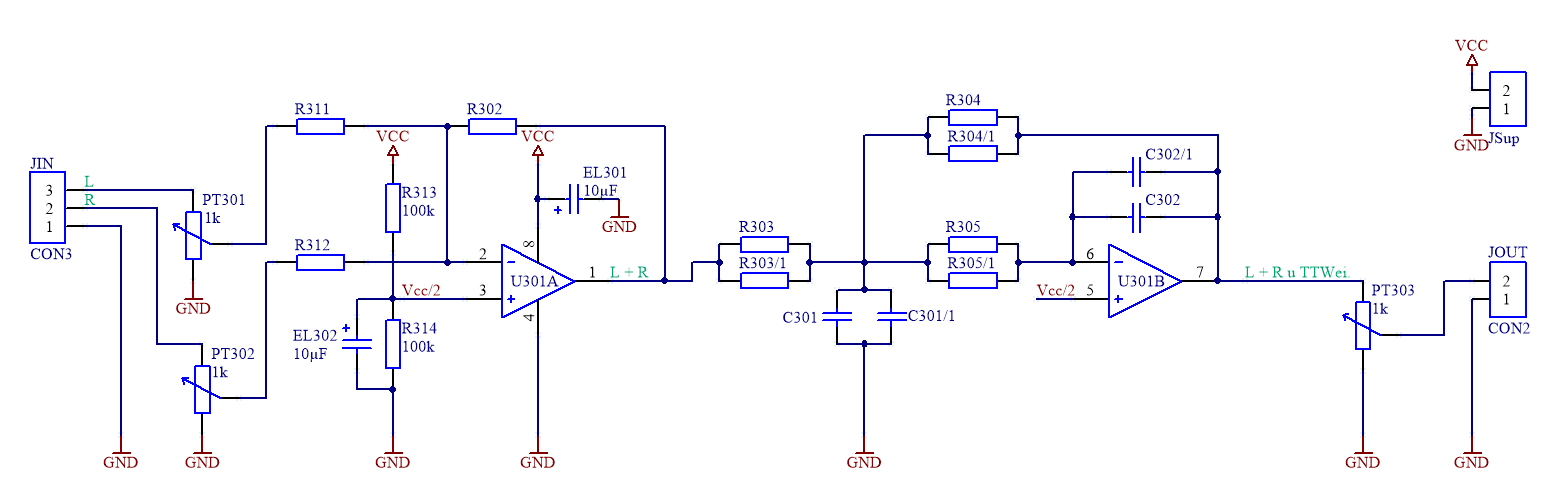
\includegraphics[width=0.8\textwidth]{img/Print3/3mTTWeicheruAddiererDiplSchematic.PNG}
	\caption{Schematic Mono-Bass-Addier-Schaltung und Mono-Bass-Weiche}
	\label {fig:4.1.3.1}
\end{figure}
\begin{figure} [H]
	\centering
	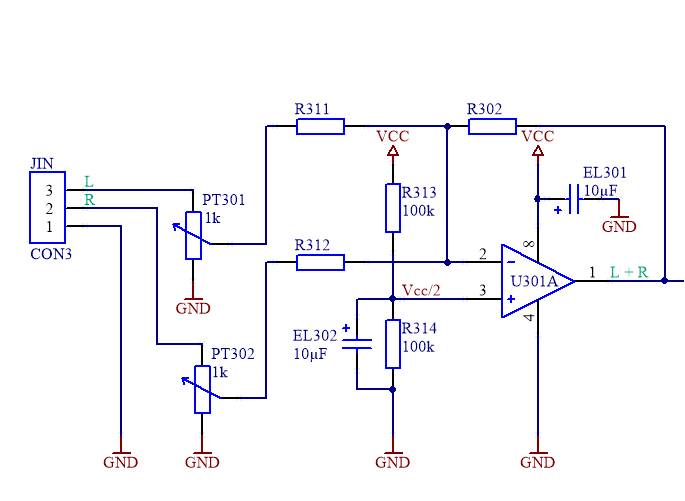
\includegraphics[width=0.8\textwidth]{img/Print3/3mTTWeicheruAddiererDiplSchematicTeil1.png}
	\caption{Schematic Mono-Bass-Addier-Schaltung}
	\label {fig:4.1.3.2}
\end{figure}
\begin{figure} [H]
	\centering
	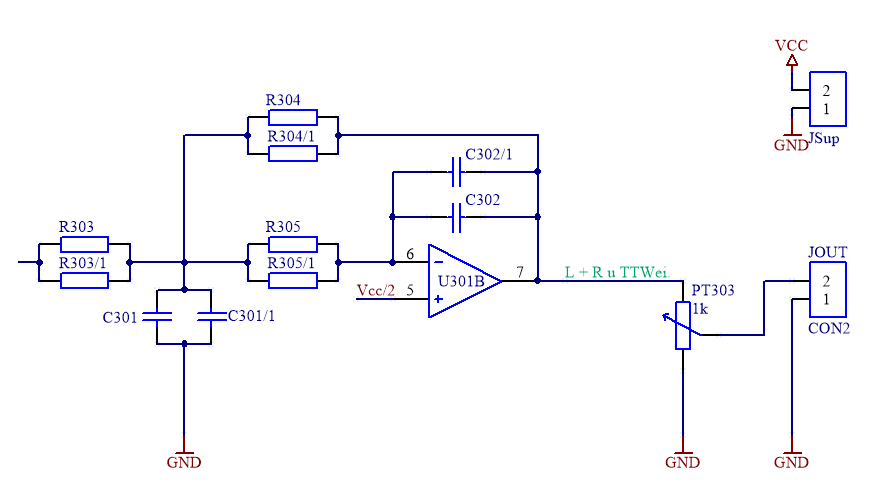
\includegraphics[width=0.8\textwidth]{img/Print3/3mTTWeicheruAddiererDiplSchematicTeil2.png}
	\caption{Schematic Mono-Bass-Weiche}
	\label {fig:4.1.3.3}
\end{figure}

\subsection{PCB}\label{subsec:4.1.4}
An einer der vier Seiten der Leiterplatte(Abb. \ref{fig:4.1.4.1})(in diesem Fall: Unten) wurden alle wesentlichen Ein- und Ausgänge platziert. Eine dreipolige Eingangsstiftleiste für Rechts, Links und Masse. Eine zweipolige Ausgangsstiftleiste für Signal und Masse. Des weiteren darf die Spannungsversorgung nicht fehlen. Wegen größeren Spannungen wurden massivere Stecker verwendet. In diesem Fall handelt es sich um steckbare Pol-Klemmen. Zum Testen wurde ein zusätzlicher Masse-Printstift angebracht um bei Messungen mit einem Oszilloskop einem besseren Massebezugspunkt zu haben.\\
Die Bauteile wurden nach Möglichkeit gestaffelt, beziehungsweise gruppiert auf der Leiterplatte platziert um den Platzbedarf zu minimieren.\\
Es wurde grundsätzlich auf jeden Print versucht eine geeignete Beschriftung vor zu sehen um Außenstehenden die Handhabung mit dem Print ebenfalls zu ermöglichen. Masse wurde selten Beschriftet, da eine Massefläche verwendet wurde und daher die Masseverbindungen sehr gut ersichtlich sind.
\begin{figure} [H]
	\centering
	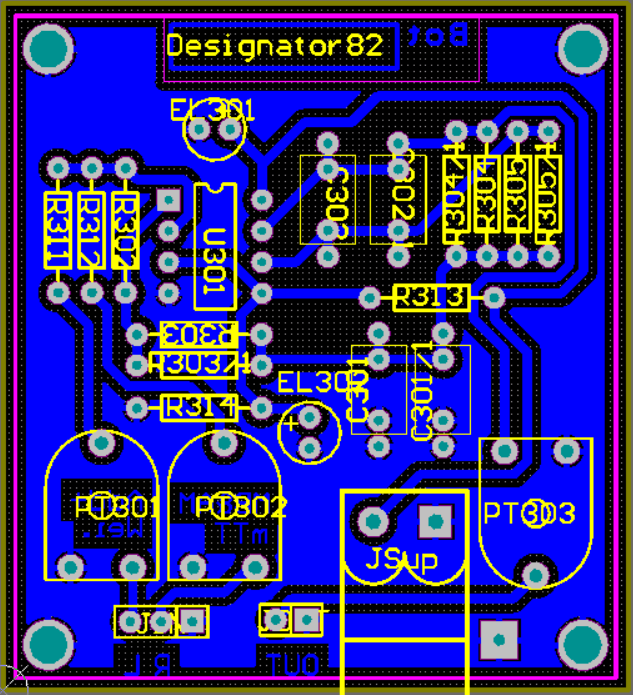
\includegraphics[width=0.8\textwidth]{img/Print3/3mTTWeicheruAddierer-PCB.PNG}
	\caption{PCB}
	\label {fig:4.1.4.1}
\end{figure}









